The Android Phone has a three direction accelerometer sensor that reads the change in speed along three axis ($x$, $y$, and $z$). 
Programs using the accelerometer read this information to give the phones orientation in space or the phones change in speed and direction. 
\\\\
In order to read this information an Acceleration object is populated and returned by any of the API's Accelerometer methods. Acceleration values include the effect of gravity ($9.81 m/s^{2}$), so that when a device lies flat and facing up, $x$, $y$, and $z$ values returned should be $0$, $0$, and $9.81$




\subsubsection{Exercise Algorithm}



\begin{figure}[H]
	\centering
		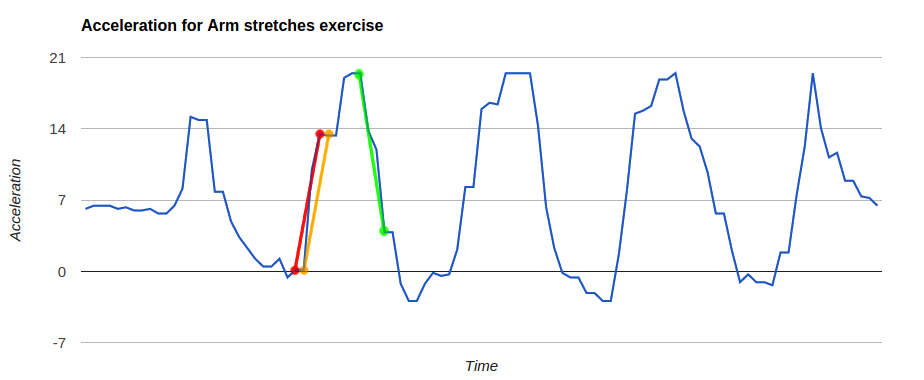
\includegraphics[width=0.80\textwidth]{images/Armstretch.png}
	\caption{Acceleration in the Y axis during the Arm Stretch exercise. The periodicity of exercises we have used provides an advantage when counting the number of finished repetitions. \textit{Up-steps} are marked in red and yellow, \textit{down-step} is marked in green.}
	\label{fig:acceleration1}
\end{figure}

Our final algorithm works by finding \textit{up-steps} and \textit{down-steps} in the acceleration values. An \textit{up-step} is defined at points where the difference in acceleration over $s$ last samples changed more than threshold $T$. A \textit{down-step} is defined at points with change larger than $-T$. 

The number of repetitions is then increased each time an \textit{up-step} appears, then a \textit{down-step} has to occur before the next repetition can be added. To counter impulsive noise, in the final version of the algorithm, we require two \textit{up-steps} to appear in two consecutive samples. The steps are visualized on Figure \ref{fig:acceleration1}.

\begin{figure}[H]
	\centering
		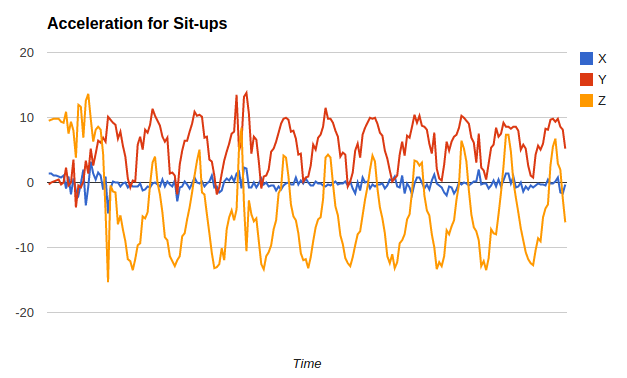
\includegraphics[width=0.80\textwidth]{images/Chart3.png}
	\caption{Acceleration in all axes during Sit-ups}
	\label{fig:acceleration2}
\end{figure}

For each exercise, we performed measurements with two test subjects and chose an axis with the highest response and a corresponding threshold. For several exercises, we combined the acceleration in two axes with the highest response, if their frequency was equivalent. An example can be seen on figure \ref{fig:acceleration2}.


\subsection{Pedometer}

To achieve the detection of steps some understanding of the walking movement is necessary. There are many parameters to describe the activity of walking such as distance, velocity, acceleration. We will use the acceleration to detect when a step is taken. We have chosen the accelerometer over GPS to allow people to walk inside the building as well, for example on their coffee break.
\\\\
When someone is walking there is some acceleration in their arms, waist, legs and feet. Acceleration of the feet is the most accurate but for the purposes of our project we will use the waist and leg acceleration since the pocket is the most obvious place for someone to have their phone and it is easy to carry that way.
\\\\
For measuring steps, we used the pedometer algorithm provided by \cite{1_berk_2014}. In short, the algorithm works by finding local minima and maxima in acceleration in the Z axis and comparing their difference to a threshold. The walking acceleration measured in one of our test sessions is presented on Figure \ref{fig:acceleration3}.

\begin{figure}[H]
	\centering
		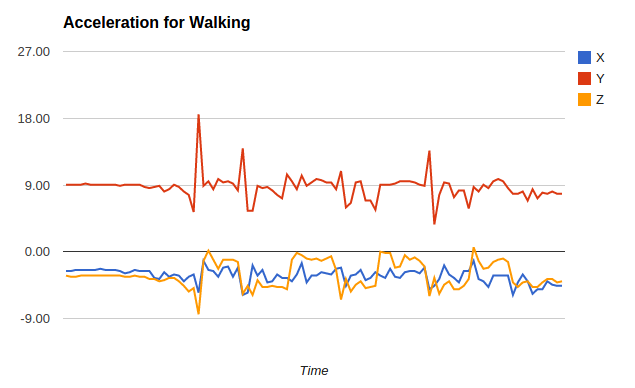
\includegraphics[width=0.80\textwidth]{images/Chart2.png}
	\caption{Acceleration of Walking}
	\label{fig:acceleration3}
\end{figure}


\subsection{Alternative approaches}

At this point it is important to explain why we chose not to get position out of the acceleration.
In order to achieve linear acceleration we need to compensate for gravity as follows:
\\\\
Linear acceleration = Accelerometer Data – Gravity
\\\\
Then we have to integrate it once to get velocity 
\\\\
$$v= \int a dt$$
\\\\
and then integrate it again to get position
\\\\
$$x= \int v dt$$
\\\\
However this method integrates noise and results to 20cm-8.5m of drift over a single second. So it is not suitable to measure our exercises since the error is much larger than the distance required to complete them.

\bibliography{sources}